\section{Discussions}\label{discussion}

Compared with the SS ADCs, the SAR/SS ADCs relatively require fewer extra control circuits for achieving adaptive-precision and take much less steps for conversion with the same bits. However, the SS ADCs inherently require less area and are easier to design. Therefore, according to specific design specifications, different architectures can be chosen. 

As for the proportion between the power off time and the conversion time, 64/78 is achieved in the SAR/SS ADCs, which is a little less than the number 240/256 in the SS ADCs. More generally, assuming the low-precision conversion is targeting $a$ bits and the full-presision conversion is targeting $b$ bits, the corresponding equations formulating the proportion of gating time for the SS ADCs and SAR/SS ADCs will be as $2^b-2^a/2^b$ and $2^{b-a}/(k*a+2^{b-a})$, where the $k$ is a coefficient describing how many extra steps are needed for the comparison with SAR logic. Further assuming $k=4$, we can plot the proportion of gating time as in Fig.~\ref{Proportion}.
%with different $a$ and $b$ for the SS ADC s and SAR/SS ADCs. 
It shows that the SS ADCs are suitable for the cases where the $b-a$ is relatively small while the SAR/SS ADCs are able to have better power scaling capability for the cases where the $b-a$ is relatively large. On the other hand, the SS ADCs oringinally have trouble converting with higher than 10 bits because exponential increasing conversion steps will unbearably limit the throuput. 
Therefore, adopting 4/8-bit adaptive-precision for the SS ADCs and 4/10-bit adaptive-precision for SAR/SS ADCs will promote strengths and avoid weaknesses for the two different achitectures, respectively.

\begin{figure}[htbp]
	\centerline{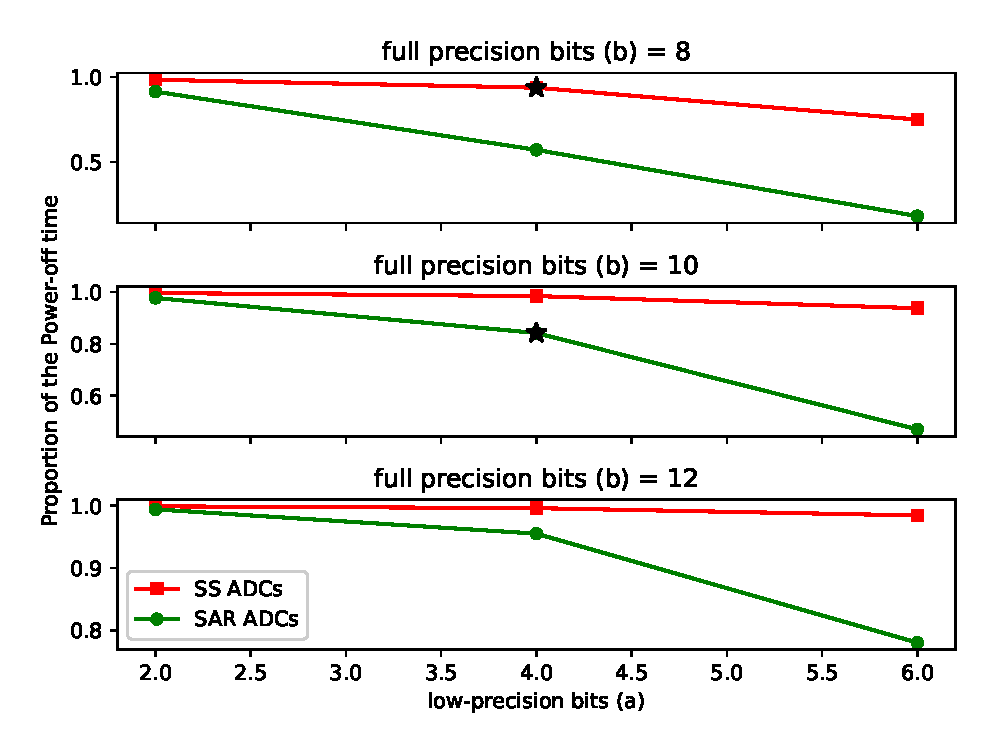
\includegraphics[width=3.5in]{./Figures/Proportion.eps}}
	\caption{Gating Time Proportion Analysis for the SS and SAR/SS ADCs.}
	\label{Proportion}
\end{figure} 

For other different precision configurations and number of parallel collumns, 
the corresponding power consumption and energy-saving performance can also be estimated with extending the evaluation results in Sect.~\ref{result}.